
By looking at \autoref{model_comparison} it can be seen that be making the simplification of the GWPL, not only loses the model applicability, as it is now necessary to calculate the conditions before assessing the the PL, but also the inaccuracy of the prediction increases. This is due to some weak points of the simplifications made. It can be seen that FSPL actually predicts quite well inside its valid region, but it is also the model that has second fewest valid points in the measurement campaign, due to the assumption of no multipath. Where TRPL has the highest valid region of the simplified models has a rather high MSE, this is due to its lack of ability to account for the surface wave, as seen from \eqref{two_ray_model} when the heights go to zero so does the power received. The NSPL is worst off, lacking in both applicability as well as accuracy, the weak point here is primarily the need of $z$. This leaves all model with crucial weak points. This paper will now propose a model that accounts for some of these weak points. 


In terms proposing a PL model six parameters is considered distance, height of Tx, height of Rx, antenna type, polarization and environment. In Appendix it is shown that there is very little correlation between signal level and antenna type, polarization and environment compared to the distance and heights, therefore those factors are deemed unnecessary to consider, which leaves only the distance and heights as needed to be considered in our proposed model. This is in expected as only the NSPL has some dependency on polarization and environment. 

This means that when designing a PL model it is reasonable build it around the existing models. The aim is to make a simple version of the GWPL model, has high applicability and high accuracy, but is still simple to calculate compared to GWPL. Therefore the as a base for the model will be the TRPL the weak point here was it inaccuracy at very low heights which could be accommodated by adding the NSPL. 

\begin{align}
Proposed model &= TRPL + NSPL \\
P_r & = \frac{P_t G_t G_r }{L}\left(\frac{h_t^2 h_r^2+h_0^4}{d^4}\right)
\end{align}

This model still suffer the weak point from NSPL of dependency upon $z$, however as only the magnitude of $z$ is needed this can be guestimated in most cases and in more critical cases it can be measured using the method described in \cite{Kim}. From our measurement the average magnitude of $z$ is 0.8122. To find out the performance of the model it is compared to the other models with the average $z$. First to analyse the applicability of the model it has the same applicability as the TRPL model which means it can be used if \eqref{two_ray_cond} is true else FSPL should still be used. The accuracy is found on the same data set as the other models as none of the data points has been used for the derivation of any part of the model. The MSE is found to 87.66.

\begin{figure}[!htbp]
\centering
% This file was created by matlab2tikz.
%
%The latest updates can be retrieved from
%  http://www.mathworks.com/matlabcentral/fileexchange/22022-matlab2tikz-matlab2tikz
%where you can also make suggestions and rate matlab2tikz.
%
\definecolor{mycolor1}{rgb}{0.00000,0.44700,0.74100}%
\definecolor{mycolor2}{rgb}{0.85000,0.32500,0.09800}%
\definecolor{mycolor3}{rgb}{0.92900,0.69400,0.12500}%
\definecolor{mycolor4}{rgb}{0.49400,0.18400,0.55600}%
%
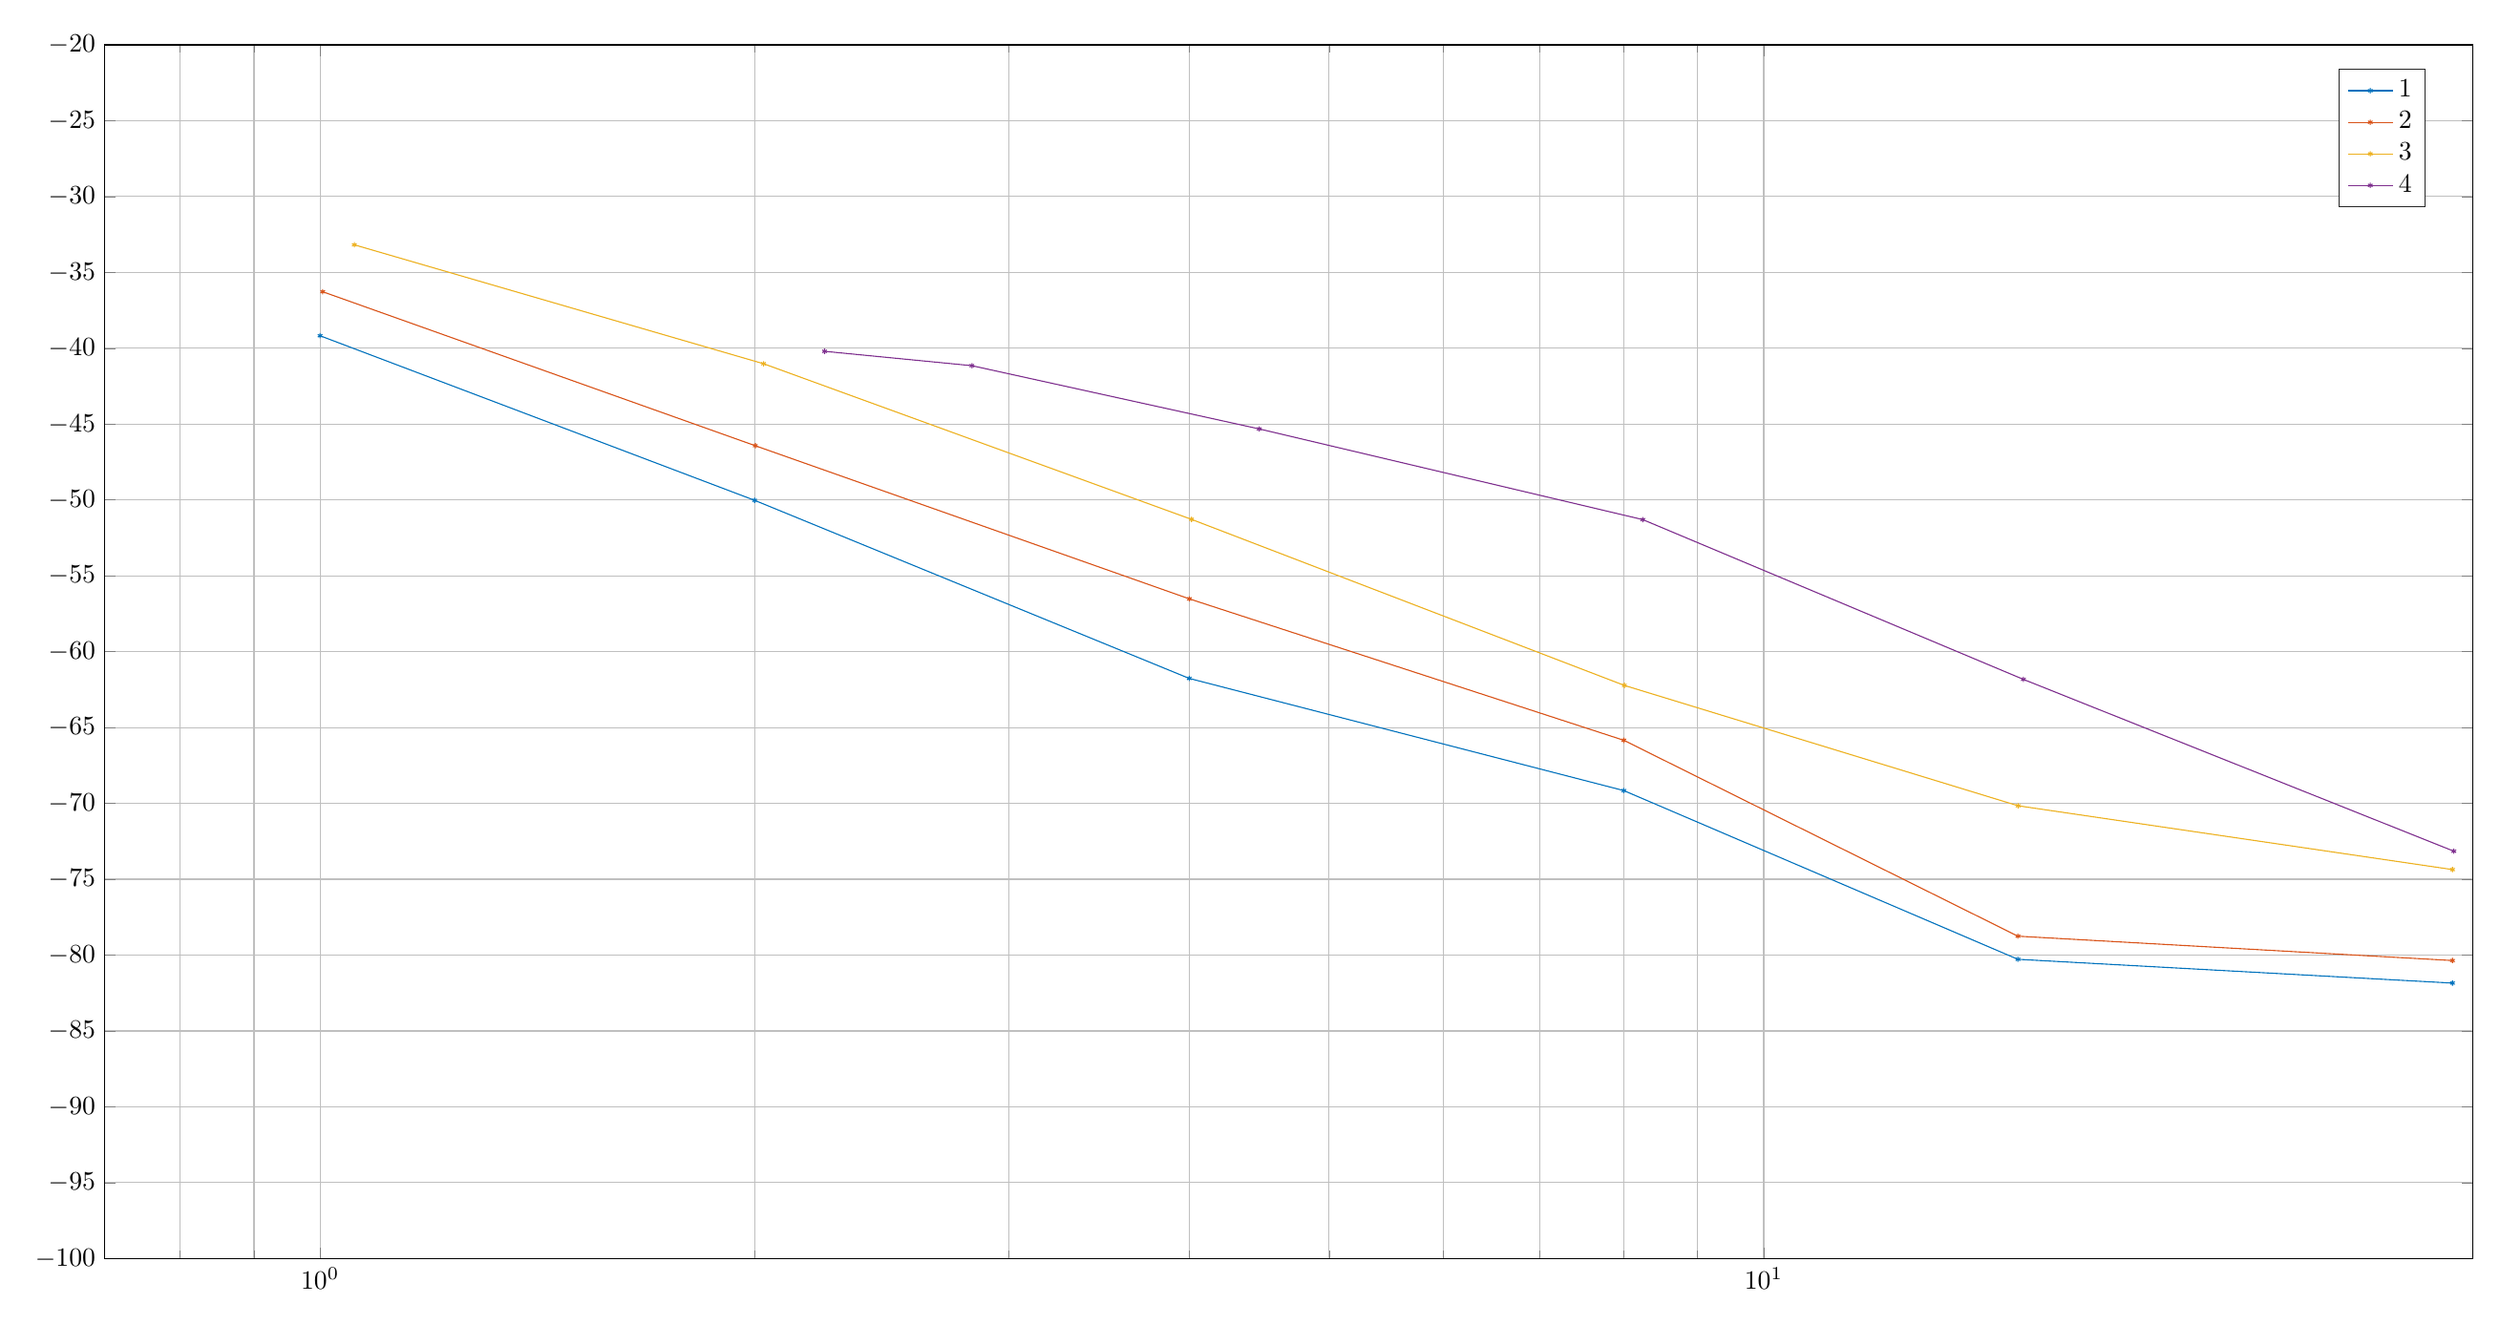
\begin{tikzpicture}

\begin{axis}[%
width=12.4in,
height=6.357in,
at={(2.08in,0.858in)},
scale only axis,
xmode=log,
xmin=0,
xmax=31,
xminorticks=true,
xmajorgrids,
xminorgrids,
ymin=-100,
ymax=-20,
ymajorgrids,
axis background/.style={fill=white},
legend style={legend cell align=left,align=left,draw=white!15!black}
]
\addplot [color=mycolor1,solid,mark size=1.0pt,mark=asterisk,mark options={solid}]
  table[row sep=crcr]{%
1	-39.176832441447\\
2	-50.0236813268286\\
4	-61.7627349006033\\
8	-69.1568155321866\\
15	-80.2784721484843\\
30	-81.8463231335614\\
};
\addlegendentry{1};

\addplot [color=mycolor2,solid,mark size=1.0pt,mark=asterisk,mark options={solid}]
  table[row sep=crcr]{%
1.00422308278589	-36.2750685665333\\
2.00211488181872	-46.4255855564945\\
4.0010578601165	-56.521087110148\\
8.00052898251109	-65.8421427417313\\
15.0002821306801	-78.7553243580291\\
30.000141066335	-80.3591753431061\\
};
\addlegendentry{2};

\addplot [color=mycolor3,solid,mark size=1.0pt,mark=asterisk,mark options={solid}]
  table[row sep=crcr]{%
1.05621967412087	-33.1826999363486\\
2.02869416127715	-41.0212571697177\\
4.01442399355125	-51.2789435665333\\
8.0072217404041	-62.2242106975379\\
15.0038528385212	-70.1578243580291\\
30.0019266048032	-74.3636753431061\\
};
\addlegendentry{3};

\addplot [color=mycolor4,solid,mark size=1.0pt,mark=asterisk,mark options={solid}]
  table[row sep=crcr]{%
2.23606797749979	-40.2024392944793\\
2.82842712474619	-41.1498149750094\\
4.47213595499958	-45.3166779228563\\
8.24621125123532	-51.29571423555\\
15.1327459504216	-61.8265071697177\\
30.0665927567458	-73.152023643832\\
};
\addlegendentry{4};

\end{axis}
\end{tikzpicture}%
\caption{Mesurements of PL for transmitter at 0.01m and receiver antenna at varying heights}
\label{Meas2}
\end{figure}

\begin{figure}[H]
\centering
% This file was created by matlab2tikz.
%
%The latest updates can be retrieved from
%  http://www.mathworks.com/matlabcentral/fileexchange/22022-matlab2tikz-matlab2tikz
%where you can also make suggestions and rate matlab2tikz.
%
\definecolor{mycolor1}{rgb}{0.00000,0.44700,0.74100}%
\definecolor{mycolor2}{rgb}{0.85000,0.32500,0.09800}%
\definecolor{mycolor3}{rgb}{0.92900,0.69400,0.12500}%
\definecolor{mycolor4}{rgb}{0.49400,0.18400,0.55600}%
%
\begin{tikzpicture}

\begin{axis}[%
width=\myvara,
height=\myvar,
at={(2.08in,0.858in)},
scale only axis,
xmode=log,
extra x ticks={2,5,20}, 
extra x tick style={log identify minor tick positions=false},
every tick label/.append style={font=\tiny},
log ticks with fixed point,
xmin=0.9,
xmax=31,
xlabel=\tiny Distance (m),
xminorticks=true,
xmajorgrids,
xminorgrids,
ymin=20,
ymax=80,
ylabel=\tiny Path loss (dB),
title = \tiny\textbf{ht = 2.02 m},
ymajorgrids,
legend pos = north west,
axis background/.style={fill=white},
legend style={legend cell align=left,align=left,draw=white!15!black,font=\tiny}
]
\addplot [color=mycolor1,solid,mark size=1.0pt,mark=asterisk,mark options={solid}]
  table[row sep=crcr]{%
2.23606797749979	40.2024392944793\\
2.82842712474619	41.1498149750094\\
4.47213595499958	45.3166779228563\\
8.24621125123532	51.29571423555\\
15.1327459504216	61.8265071697177\\
30.0665927567458	73.152023643832\\
};
%\addlegendentry{hr = 0.04m};

\addplot [color=mycolor2,solid,mark size=1.0pt,mark=asterisk,mark options={solid}]
  table[row sep=crcr]{%
2.1541736234575	40.5286184873639\\
2.7641389255969	41.7634386176021\\
4.43175631099003	43.3569736894665\\
8.22438228683468	49.22358923555\\
15.1208618801972	58.5868821697177\\
30.060613167399	67.725648643832\\
};
%\addlegendentry{hr = 0.14m};

\addplot [color=mycolor3,solid,mark size=1.0pt,mark=asterisk,mark options={solid}]
  table[row sep=crcr]{%
1.93793704748116	37.947787309918\\
2.59915370842126	41.5490546940608\\
4.33077360294902	43.1688945864033\\
8.17041002643074	46.5688884715957\\
15.0915738079234	52.6026681377669\\
30.0458915660694	64.022898643832\\
};
%\addlegendentry{hr = 0.36m};

\addplot [color=mycolor4,solid,mark size=1.0pt,mark=asterisk,mark options={solid}]
  table[row sep=crcr]{%
1	28.6391813268286\\
2	35.8754849006033\\
4	42.4804405321866\\
8	48.4989721484843\\
15	51.0989481335614\\
30	59.847479174472\\
};
%\addlegendentry{hr = 2.02m};

\end{axis}
\end{tikzpicture}%
\caption{Mesurements of PL for transmitter at 2.00m and receiver antenna at varying heights}
\label{Meas3}
\end{figure}



%The reasoning behind adding exactly these two models is that the TRPL and NSPL overlap each other, given there conditions, where if the purposed model included FSPL, then the TRPL is not valid where FSPL is valid. 

%both takes into account the direct and reflected wave, while the NSPL, takes into account the surface wave. This is given for the conditions that the two models have to uphold \eqref{cond_surface}, \eqref{two_ray_cond}.

%As both the TRPL and NSPL have their conditions these same conditions will be applied to the our purposed model. 
%When comparing the MSE and coverage are of our purposed model and the GRPL, where the MSE of our purposed model is 65.42, while the coverage is 65.00$\%$. The MSE of the GRPL is still better.  \\


%The measurements at the smallest distances between the transmitter and the receiver, will suffer from not being in the Far Field, this could indicate why some of the measurements behave as they do. \\

%Also other measurements at different distances have a weird jump this could involve an environmental factor, as also the measurments have been done over three days, at the parking lot. 
     
